\begin{figure}[!htb]
\begin{center}
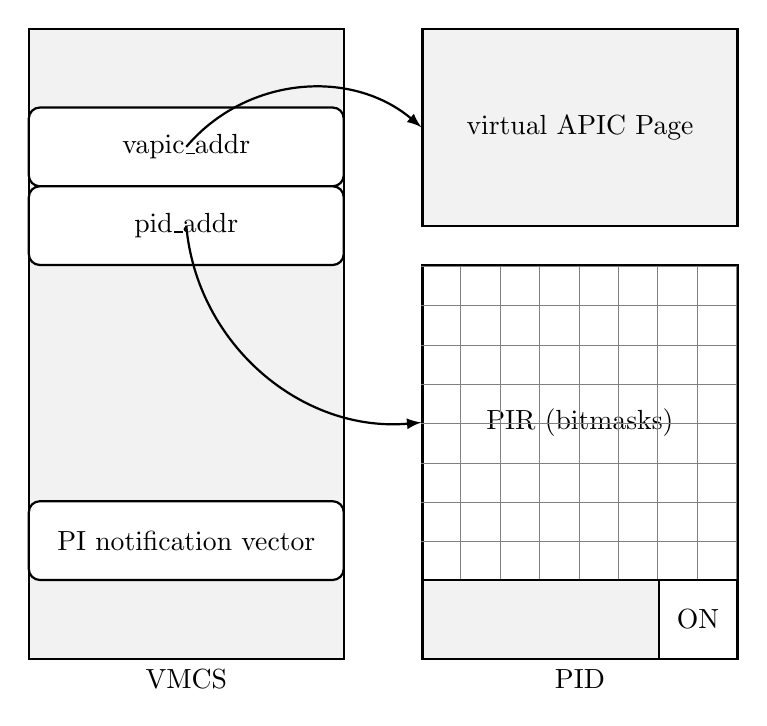
\begin{tikzpicture}


%%\draw[step=0.5cm, gray, very thin] (0,0) grid (9,9);

\node at (0,0) [rectangle, draw=black, thick, fill=black!5, minimum height = 8cm, minimum width = 4cm, anchor=south west] (vmcs) {} ;
\node [below, align=center] at (vmcs.south) {VMCS};

\node at (0,6) [rectangle, draw=black, thick, fill=white, rounded corners, minimum height = 1cm, minimum width = 4cm, anchor=south west] (apicaddr)  {vapic\_addr};
\node at (0,5) [rectangle, draw=black, thick, fill=white, rounded corners, minimum height = 1cm, minimum width = 4cm, anchor=south west] (pidaddr)  {pid\_addr};

\node at (0,1) [rectangle, draw=black, thick, fill=white, rounded corners, minimum height = 1cm, minimum width = 4cm, anchor=south west] (pinv)  {PI notification vector};

\node at (5,1) [rectangle, draw=black, thick, fill=white, minimum height = 4cm, minimum width = 4cm, anchor=south west] (pir) {PIR (bitmasks)};
\begin{scope}[fill opacity=0.9]
	\draw[xstep=0.5cm, ystep=0.5, gray, very thin] (5,1) grid (9,5);
\end{scope}

\node at (5,0) [rectangle, draw=black, thick, fill=black!5, minimum height = 1cm, minimum width = 4cm, anchor=south west] (rsrvd) {};
\node at (8,0) [rectangle, draw=black, thick, fill=white, minimum height = 1cm, minimum width = 1cm, anchor=south west] (on) {ON};
\node [below, align=center] at (rsrvd.south) {PID};

\node at (5,5.5) [rectangle, draw=black, thick, fill=black!5, minimum height = 2.5cm, minimum width = 4cm, anchor=south west] (vapic) {virtual APIC Page};


\begin{scope}[>=latex]
	\draw [thick, ->] (apicaddr.center) to [bend left=45] (vapic.west);
	\draw [thick, ->] (pidaddr.center) to [bend right=45] (pir.west);
\end{scope}


\end{tikzpicture}
\end{center}
\caption{Key data structuers for Posted Interrupt processing. Virtual APIC page is used by VT-x to virtualize interrupt controller memory accesses. 
PINV is interrupt vector number that uses PID data structure for delivery without exit.
PID consists of ON bit and PIR bitmasks. Host marks PIR bit corresponding to interrupt vector and sets ON bit
to deliver interrupt direclty to guest.}
\label{fig-pi-ds}
\end{figure}
